
\documentclass[10pt]{article}
\usepackage[utf8]{inputenc}
\usepackage{geometry}
\usepackage[english]{babel}
\usepackage{natbib}

\usepackage{graphicx}
\graphicspath{ {./assets/} }

\geometry{
  a4paper,
  margin=1in
}
\linespread{1.5}

\usepackage{hyperref}
\hypersetup{
    colorlinks=true,
    linkcolor=blue,
    filecolor=magenta,      
    urlcolor=cyan,
}
\urlstyle{same}

\usepackage{tocbibind}

\title{Deliverable 1}
\author{Alfie Richards, Joe Cryer, Patrick Cooke, Adam Price, Arnau Ayerbe Garcia}

\begin{document}
\date{November 2020}
\maketitle
\tableofcontents

\newpage

\section{Domain}
\subsection{Background}
\subsubsection{What is the domain}

The domain chosen has been American Sign Language,it is the predominant language of Deaf 
communities. This language is used by many people daily however there exist a large number of 
dialects as well as difficulties in learning sign language. For example, British Sign Language is 
not the same as American Sign Language and there does not exist a universal language. American Sign 
Language is a different language to the ones you may think of usually, unlike when having a 
conversation in English with someone the use of voice has no impact due to the fact it is designed 
to be understood by deaf people. Letters and therefore words are pronounced using hand gestures. On 
the other hand, American Sign Language has variations depending on the person who is speaking 
similar to when people have different accents. 
\cite{national_institute_of_deafness_and_other_communication_disorders_2020} .This can make it 
difficult to grasp at first, for some people who are new to the language or the difference is too 
big in comparison to other spoken languages. 

Overall sign language is key for our society, we as human beings rely heavily on communication with 
one another. Sign language allows people with impaired hearing to communicate with other people in a 
much better way. Although it is not always that easy, as sign language is not known by everyone,so 
sometimes it can be very difficult to understand what another person is trying to tell you. With all 
of this being said, the statistics are astonishing, 11 million people are deaf or hard of hearing in 
the UK, that makes around 16.7\% of the population has hearing difficulties . Nonetheless there are 
only around 150,000 British Sign Language users, this shows clearly the dilemma they are facing. As 
a consequence of this people with hearing difficulties are more prone to unemployment and mental 
health issues. \cite{gov.uk_2019}. You could argue one obstacle leads to the other, yet they are 
both urgent problems to solve.

\subsubsection{Motivation}

Because of this on the transition to a much-more online world the need for interpreting sign 
language is necessary for things such as online doctor service or simply online video call 
communication. As the hardship of lockdown and isolation affects everyone, it impacts Deaf people 
the most, a vulnerable population which already suffered from loneliness as mentioned earlier has 
seen the risk of this mental health condition rise. The option of speaking to friends or family 
members over the phone is much less feasible for them for obvious reasons. In like manner Deaf clubs 
have being forced to shut down during long periods, they appear a place where they can socialise and 
stay in contact, the changeover to online meetings in the best cases has being hurtful for the 
community \cite{heren_2020}.The benefits from technology can be used to help, understanding ASL may 
be very challenging at first; this can be minimised. Undoubtedly the need for this has increased 
exponentially over the last few months \cite{kalia_2020}, during these unprecedented times we are 
living where COVID-19 has influenced our lifestyle. Online communication is one of the biggest 
challenges, here we can find a clear example of how without an interpreter you would have to text 
chat with one another. This is far from ideal and can be solved. 

In addition to this, the other main form of communication for a Deaf person is lip-reading 
\cite{hearing_dogs_for_deaf_people}, while this is a harder and less accurate form of communication 
it is currently becoming obsolete due to the Government guidelines regarding the COVID-19 pandemic, 
the issue being the required use of face coverings in enclosed spaces. For this reason, lips are 
covered by the face covering and are no longer readable, likewise, one other action we must perform 
to protect each other from the spread of the virus is social distancing with at least 1 metre (when 
using a face covering) \cite{gov.uk_2020}. Lip readers rely heavily on any residual hearing they may 
have left to interpret a conversation; with the use of face coverings and social distancing the 
difficulty of recognising any residual hearing has increased greatly and hence the struggle to 
communicate with any other person. 

Moreover the lack of existing systems allow us to explore the broad topic of a American Sign 
Language interpreter. During our research we encountered some different ideas of interpreting Sign 
Language, despite this some of them weren't complete, alternatively one other system we found 
required the use of specific technology which consisted of a glove with in-built sensors. 
\cite{mehdi_khan_2002}. Our objective is to try and simplify the process through which Sign Language 
interpretation happens as the limited access to specific equipment can minimise the scope of the 
solution. This motivated us forward to design a system which is easy to use and using common daily 
technology. 

\subsubsection{Other ideas}

During our brainstorming we took into account several different ideas and problems, we started by 
trying to find a problem in a specific domain and then thinking of a solution. The process was 
narrowed to our current proposal and a Student Hub for the students at the University of Bath, where 
they could engage and connect with other students. In our selection process we concluded the 
American Sign Language Interpreter would be more beneficial and contribute to a larger amount of 
people. At first we explored the option of doing a British Sign Language Interpreter, finally we 
chose the American Sign Language Interpreter as it has a better and larger data set which we can 
work with. Also it is spoken with only one hand. This is important as the other hand can be used to 
hold the device with the camera and record making things easier to use. 

\subsection{Understanding the Domain}

Looking into the described domain, there exists very little in terms of systems that can understand 
or interpret ASL. The closest system we could find to manage the problem presented in the domain is 
software that can have text input into them and they will return a series of images that show how to 
sign out the words or phrases \cite{handtalk}. Due to the lack of already existing solutions to the 
problem presented in the domain, this significantly increases the usefulness of our solution due to 
sparsity.

The people working on this project do not have a hearing disability, nor do they actively interact 
with someone who does, as a result they do not need to use ASL on a regular occasion. As well as 
this, nobody who is working on this project is fluent in ASL, with some group members not knowing 
any of the language. We also presented these questions to our cohort and the majority of our fellow 
students were in the same position. With these statistics it ha presented a possible need for a 
quick solution for someone who was suddenly presented with the challenge of being in a conversation 
with someone using ASL to communicate, as such we believe this presents a need for our solution to 
the given domain.

Through communicating we have made engagement with potential stakeholders into our system, as anyone 
could find themselves being in a conversation with someone who uses ASL as a main method to 
communicate. Because of this, it is clear that our stakeholders in this system are anyone, but 
mainly people who use ASL to communicate or people who don't know ASL but are likely to have to use 
it to communicate.

The experience that we do have in the domain is from past experiences, largely in employment, where 
a member of the public has come to speak to us using sign language and due to us not being fluent in 
the language we have struggled to communicate with them. Although this presented an issue for us at 
the time we can see how it would present a much greater issue for people who regularly use sign 
language to communicate and are unable to do so due to those around them not being fluent. This 
combined with the new normal of a virtual workplace can present even further frustration on those 
who rely on ASL as their main method of communication, as having to type messages to communicate can 
really slow down productivity.

With all these issues considered and combined, our group believes there exists a need for the 
solution presented below.

\subsection{Solution Proposal}

Our proposed solution for the domain that we have previously outlined is a system that takes live 
video input from a phone camera or webcam of someone communicating using ASL, it will then interpret 
what was said and return the corresponding English letters or words that were signed to the user.

We understand that the technical requirements of this solution may require some complex algorithms 
to be implemented, so we see the scope of what ASL can be interpreted as being a limiting factor. 
Because of this we will likely set our initial scope for this project to be able to interpret the
26 signing motions that make the ASL alphabet, with the accuracy of the interpretation being high.
If we have more time to expand on this scope towards the end of the project we will look into this 
depending on how feasible it may be.

A further limiting factor we have noticed is that we have set our initial scope for the system to be 
able to interpret American sign language (ASL), rather than British sign language (BSL), this was 
another choice based on the technical complexity of this project. Firstly, the ASL alphabet only 
uses one hand whereas the BSL alphabet uses two hands, so we made the choice of using ASL as the use 
of one hand will make it easier for the computer vision aspect of our system to accurately 
distinguish the different signs. Secondly, upon an initial search into the feasibility of this 
project we were able to find a much larger data set for the ASL alphabet than we were for the BSL 
alphabet, meaning that it would be easier to train our system and it would produce much more 
accurate results. 

Since our system will require no user logins or stored personal data, it will be completely fine to 
use legally as it complies with laws such as GDPR and the Data Protection Act. As well as this, 
since the proposed system won't store any of the recordings taken once the ASL has been interpreted, 
it will stand on positively ethical ground for its users.

We think that our proposed system will have a positive commercial impact, as one of the issues 
within our domain that was highlighted was the fact that people with hearing disabilities often find 
it hard to find people who understand ASL when in public, such as in bars or shops. As such we 
believe that our solution will help these people overcome this burden and make it easier for them to 
return to shops or other commercial establishments.

\section{Programme and Methodology}
\subsection{General Aims}

At the core of the project are a set of general aims and objectives. These objectives exist to 
shape the rest of the project and ensure that the original vision of the project is kept to. These 
are: 

\begin{itemize}
  \item To create a system that facilitates easier communication between English speaking and ASL 
    non-verbal communicators
  \item To create an intuitive user interface that is accessible and user-friendly for all 
    stakeholders
\end{itemize}

These general aims will help to guide our project, and are expanded upon more within our milestones.

\subsection{Milestones}

There are a set of milestones that serve to give us structure for our development cycles and 
inform us of our progress. These milestones mark major feature progression within our project, and 
help to lay out our overall vision for our solution.

\begin{itemize}
  \item Plan for system structure and stack (Second deliverable)
  \item Plan for letter recognition library (Second deliverable)
  \item Proof of concept Python system implementing a machine learning letter recognition model, 
    taught on the ASL Alphabet dataset \cite{asldataset} (2nd week of Semester 2)
  \item Generalising proof of concept system into a Python library implementing the model (2nd week 
    of Semester 2)
  \item Server side API model to allow connections to the ML model (5th week of Semester 2)
  \begin{itemize}
    \item Secure client-server authorisation implementation
  \end{itemize}
  \item Client app that hooks into the server side API and displays the responses (5th week of 
    Semester 2)

\end{itemize}

As our system utilises quite complex technologies, we intend to prototype a working solution early 
on in our development, and then build on that prototype. This is contrary to a normal development 
process (where the development of the system itself would coincide with the development of the user 
interface), but makes sense for our proposed system as a proof of concept allows functionality to be 
tested and built upon quickly. 

Our server-side and client-side systems are being developed largely in isolation from one another, 
with an API connecting the two. In order to avoid any confusion about the API - the overlap between 
the two systems -  we will create a detailed schema and documentation for the REST API before 
creating it, so that the server can be built to that specification while the client can be built 
expecting the server to follow it. All of this allows for much easier parallel development with 
multiple developers, as both sides can easily write the code for connecting to each other in 
parallel without one having to wait on the other. Obviously once both sides are created, there will 
be an in-depth testing process to work through, but we can use tools such as Postman to simulate API 
calls in the meantime. 

\subsection{Stakeholder Engagement Methods}

As outlined in the introduction we plan on interviewing and surveying our stakeholders to get 
feedback from them on the project. We will do this at multiple stages of the project, we will use 
the feedback to assist in the planning of the project as well as to get feedback for the project 
while it is in development. This will allow us to see what is working and change our plan and 
direction if needed. This is especially important for our goal of making the project accessible and 
user friendly for all stakeholders.

\subsection{Project Management}

We plan to use the agile methodology approach to development. The self organisation aspects of agile 
will be especially important given the fact we will most likely have to do most (if not all) 
development remotely this year. We will most likely use scrum to structure our development as our 
team is the right size and a lot of our team is familiar with it from the CSED module last year.  We 
will use Jira as the platform for organising scrum, as this will allow us to assign tasks, features 
and bugs to team members and track the progress for the features and towards the milestones. We will 
only use the Jira for tasks related to development - other tasks and admin related to the 
deliverables will be handled by assigning tasks in weekly meetings after the sprint reviews.

To allow collaboration within the project we will use git for version control with three individual 
repositories. The first repository will be for the client side app. The second repository will be 
for the library which recognises the alphabet from video clips. The last repository will be for the 
server which serves the REST API, and will use the library to serve requests from the app. For this 
reason the server repository will have the other two as dependencies. We will host the remote 
repositories on GitHub as it has a great feature set for collaboration and we are all familiar with 
it.

We will use the main branch on each repository as the deployment branch. This allows us to use 
GitHub actions to set up the repository to automatically deploy each branch when the main branch is 
updated. This continuous integration setup will allow us to develop faster, spending less time on 
deployment. We will also include a way for everything to be run locally so that testing and 
development can be done without having to deploy to the server - this will allow for the hosted 
version to always be reliable.

On each repository we will set up branches for each feature and bug corresponding to the features 
and bugs on the Jira. This organisation will allow for easier collaboration between teammates and 
allow us to assist each other if one of us has become bogged down on any individual task.

We will use pull requests to manage the merging of features and branches into the main branches. We 
can then use that for code reviews at each sprint review. This will help maintain code quality in 
the project and help us all stay up to date with each other's work.

\subsection{Iterative Development}

As we are using scrum we will be using iterative development. This is ideal as we will need to build 
quickly to our initial requirements. We can then add our stretch goals and additional features if 
time allows. This is especially important for this project as we are unsure how long a lot of these 
sections of the project and features will take as we will be using various technologies for the 
first time. 

The use of continuous integration will greatly assist the iterative development style as it 
encourages more, smaller iterations.

We will also build a set of unit tests for the project. Then we can run the unit tests before any 
build is submitted to the main branch. This should make our project more reliable and allow for 
quicker more frequent testing. While this will take a lot of time early in the project, it will save 
time overall and make the final project better.

\subsection{Data collection and data set}

We intend to collect no personal data from the users of the app, as this is unnecessary for our 
project. However we would like to allow for users to opt-in to allowing us to save their input on 
the server to allow us to train the ML model further. 

We have found a very good and large data set of American Sign Language alphabet images with which we 
can train our ML model. This will allow for the model to get more accurate over time.

\subsection{Software stack}

We have decided on using a mobile web app stack. This is primarily because we want to have the power 
of a server to drive the machine learning algorithm, rather than relying on mobile processors. 
Additionally there is the possibility we could train the ML model further with feedback from users 
to get more accurate over time.

For the stack we are going to use React Native for the client, as it is a multi-platform solution 
reducing the development time for multiple operating systems. Additionally as the processing will be 
done on a server the speed loss of not using native platforms isn't a concern.

For the API and server we intend to use Python Lambdas hosted on AWS. The first reason for this is 
because we learnt Python in Principles of Programming the whole team will be familiar with it. 
Another reason is Python Lambdas are easy to set up on Amazon Web Service so we can get a proof of 
concept quickly. We chose AWS because we get a free tier as students, which, when combined with the 
widespread support and reliability, makes AWS a very attractive option.

We plan to use Python for the recognition library. This is because of Python's popularity for 
machine learning and computer vision. We plan to use the OpenCV library as the base of our computer 
vision and the TensorFlow library for the ML model, both of which have first class support for 
python.

We have decided on using a mobile web app stack. This is primarily because we want to have the 
power of a server to drive the machine learning algorithm, rather than relying on mobile 
processors. Additionally there is the possibility we could train the ML model further with 
feedback from users to get more accurate over time.

For the stack we are going to use React native for the client, as it is a multiplatform solution 
reducing the development time for multiple operating systems. Additionally as the processing will 
be done on a server the speed loss of not using native platforms aren't a concern.

For the API and server we intend to use Python Lambdas hosted on AWS. The first reason for this is 
because we learnt python in Principles of Programming the whole team will be familiar with it. 
Another reason is python lambda functions are easy to setup on Amazon Web Service so we can get a 
proof of concept quickly. We chose AWS because we get a free tier as students, which when combined 
with the widespread support and reliability, makes AWS a very attractive option.

We plan to use python for the recognition library. This is because of pythons popularity for 
machine learning and computer vision. We plan to use the OpenCV library as the base of our 
computer vision and the Tensor flow library for the ML model, both of which have first class 
support for python.

\section{Work Plan}

The Gantt chart covers the entire development for the project and shows the dependencies between 
tasks for each deliverable. It was more appropriate to create a Gantt chart over a PERT chart for 
our proposed system. This is because Gantt chart allows having an overview of both time frames and 
dependencies for tasks in a linear bar chart style . Whereas a PERT chart would focus more on the 
dependencies of tasks. The Gantt chart, in conjunction with Jira, will be used to handle time 
management and the handling of tasks.

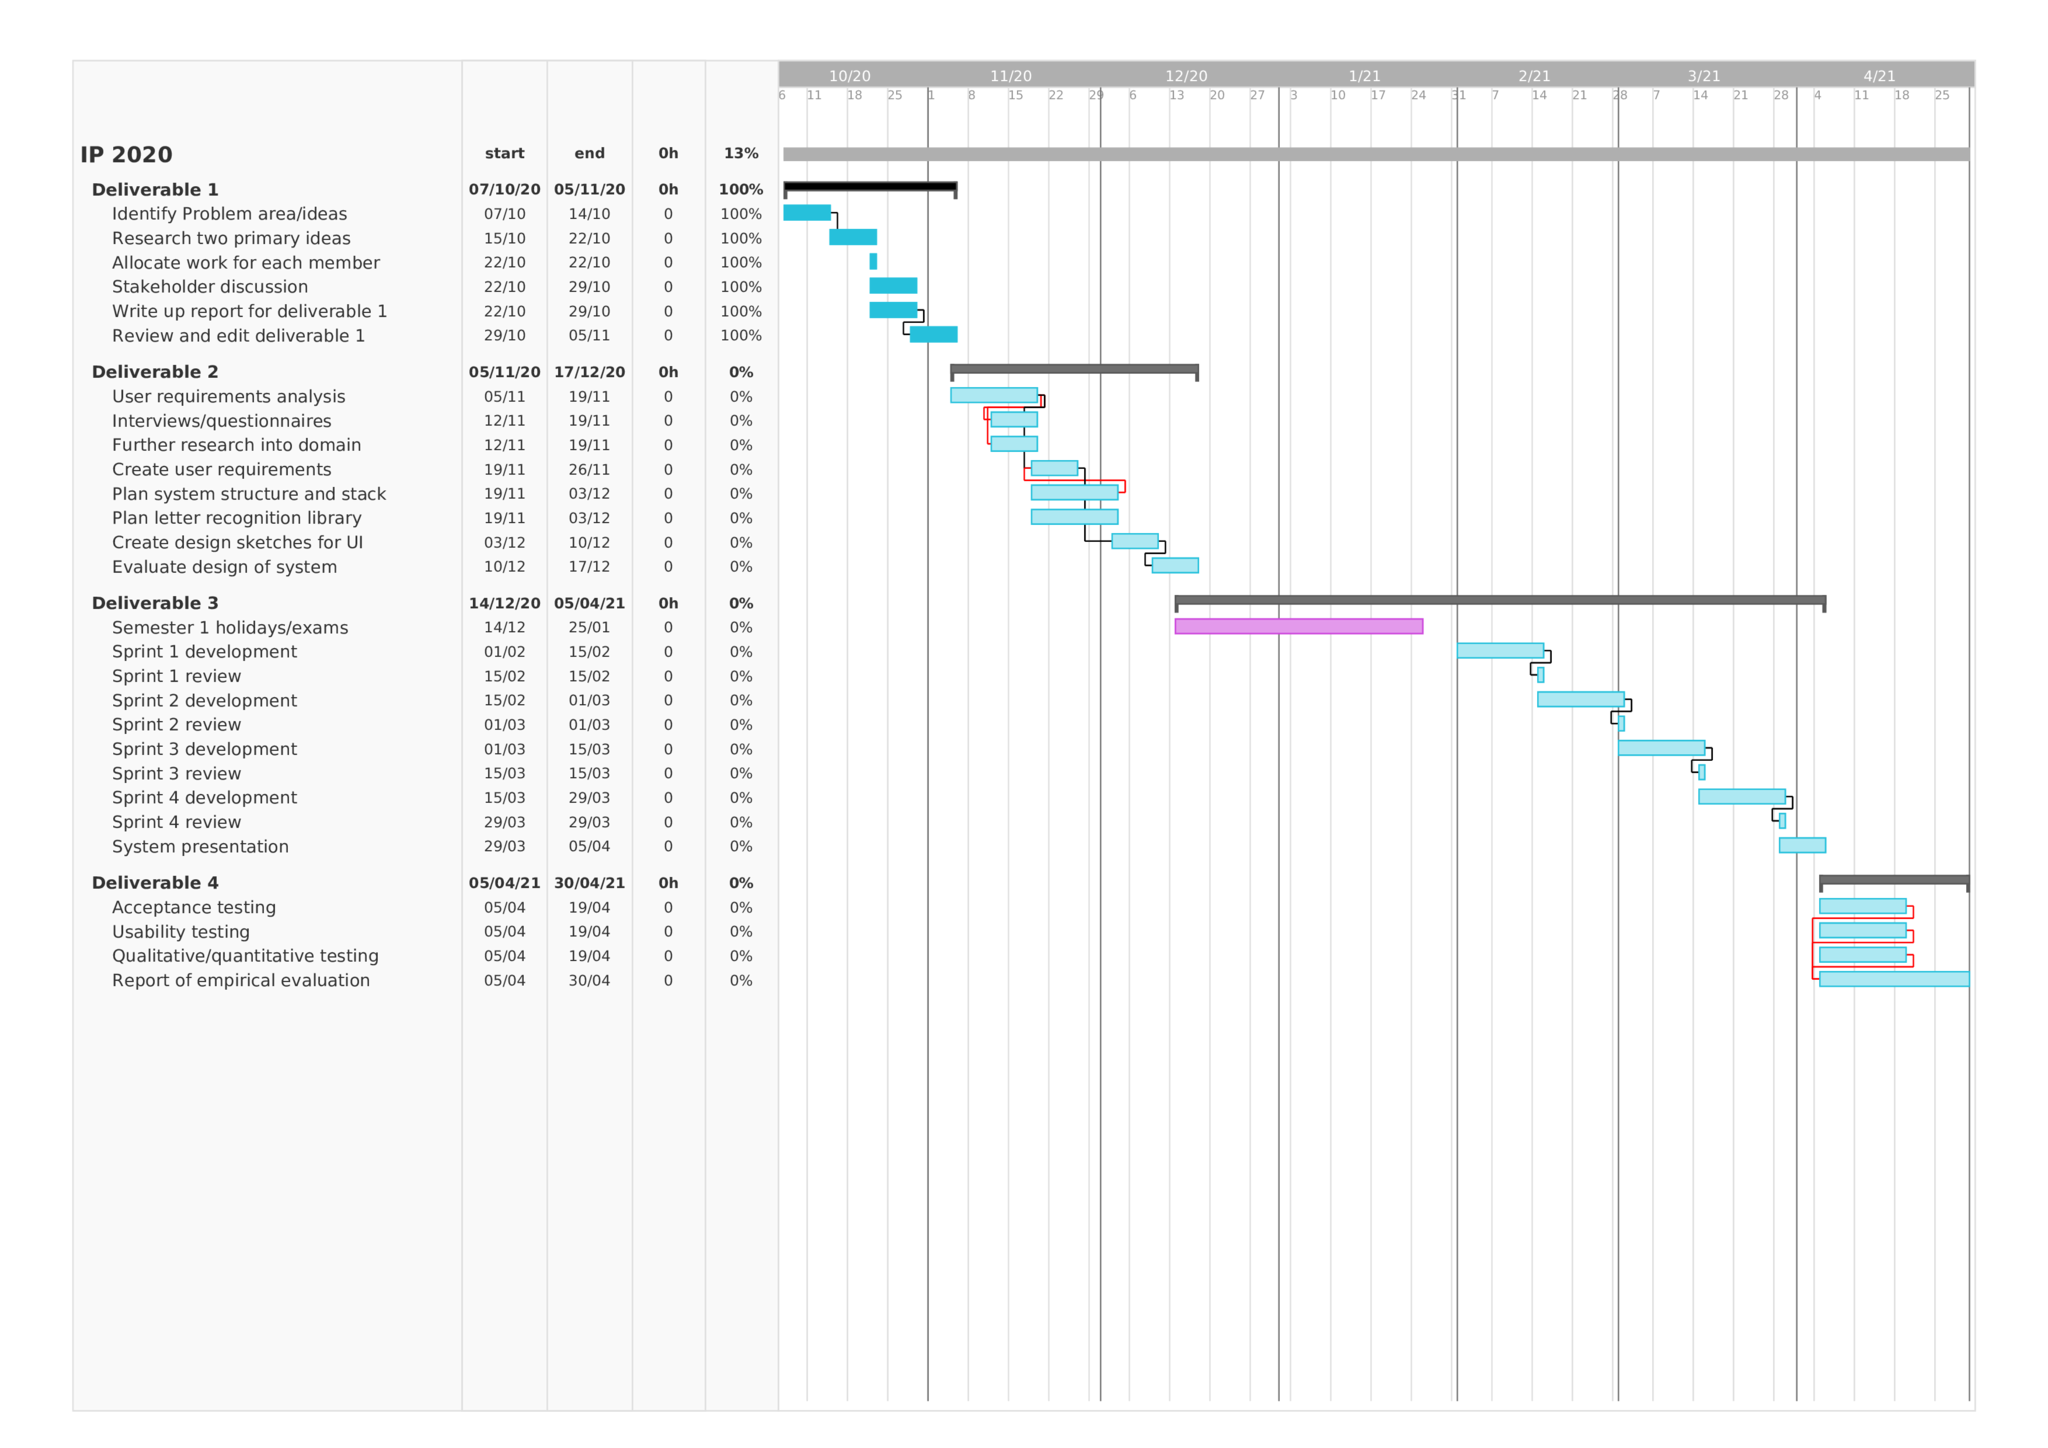
\includegraphics[width=\textwidth]{IpGantt.png}

\newpage

\bibliography{sample}
\bibliographystyle{bath}

\end{document}

